\chapter{Распределенная микросервисная архитектура генерации изображений}
\section{Распределенная микросервисная архитектура генерации изображений}
Исходя из перечисленных требований в предыдущей главе архитектура должна:
\begin{enumerate}
    \item Предоставлять возможность горизонтального масштабирования каждой из частей системы по отдельности.
    \item Предоставлять возможность инструментации для диагностики и сбора статистики.
    \item Использовать сетевой транспорт, который обеспечивает отказоустойчивость и оптимальные тайминги сетевых запросов.
    \item Позволять переиспользовать отдельные компоненты другим системам.
\end{enumerate}

В рамках данной работы была реализована система для инференса изображений с HTTP API для внешних потребителей (рис. \ref{fig:design}).

\begin{footnotesize}
\begin{figure}[H]
  \centering
  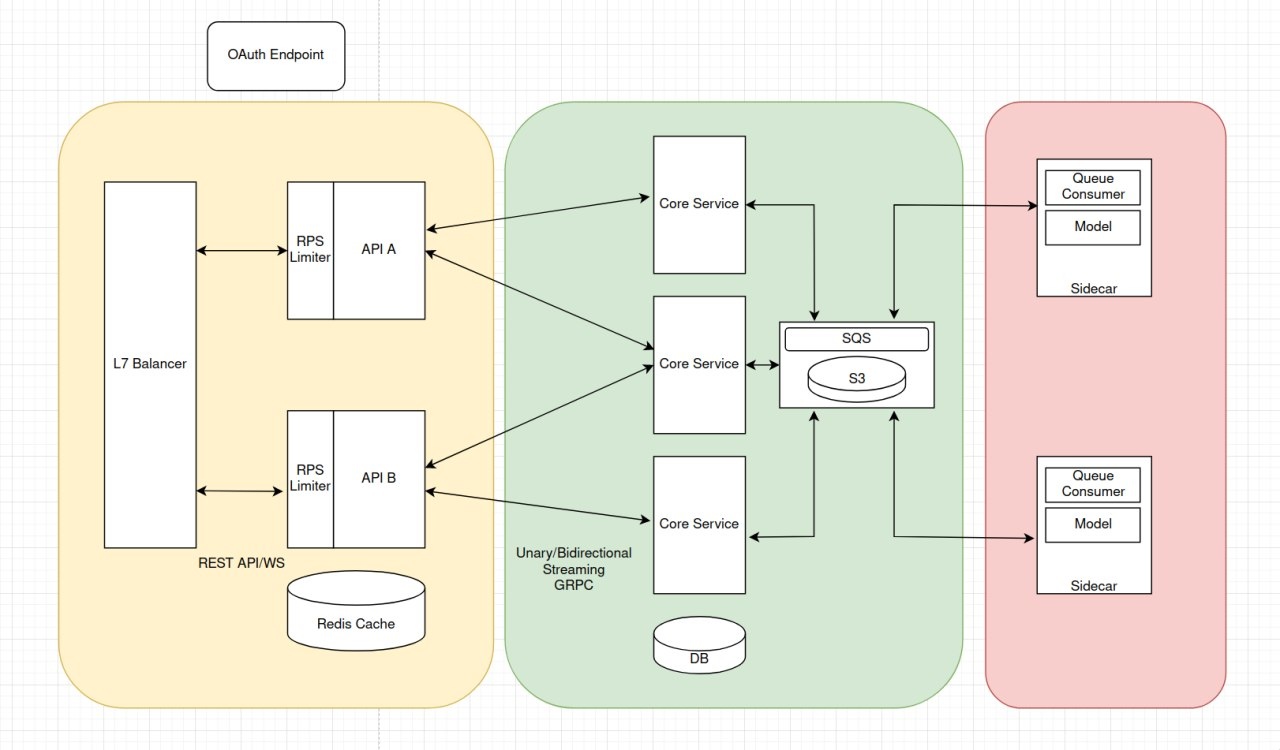
\includegraphics[width=0.95\textwidth]{img/design.png}
  \caption{Схема архитектуры}
    \label{fig:design}
\end{figure}
\end{footnotesize}

Данная система состоит из трех основных частей:
\begin{enumerate}
    \item HTTP Gateway для принятия внешних запросов.
    \item Изолированный backend с холодным хранилищем пользовательских запросов генерации.
    \item Сайдкар генерации с моделью генерации изображений с помощью нейронной сети.
\end{enumerate}

HTTP Gateway, представленный желтой зоной на рисунке \ref{fig:design}, предоставляет внешний слой приложения, который отвечает за бизнес-логику,
работу с пользовательскими данными и идентификаторами и проксирует GRPC запросы походами в основной backend.
Как правило, данная часть является наименее нагруженным компонентом системы, поэтому может быть 
представлена единичными экземплярами в каждой из локаций, известных L3 балансеру приложения.

Изоляция данного слоя также позволяет разделять источники траффика в систему и вводить разные
правила на количество поступающих запросов и отдельно кэшировать ответы основного бэкенда.

На данном слое также представляется возможным размещение документации для разработчиков, которые работают
с внешним API системы (рис. \ref{fig:swag}).

\begin{footnotesize}
\begin{figure}[H]
  \centering
  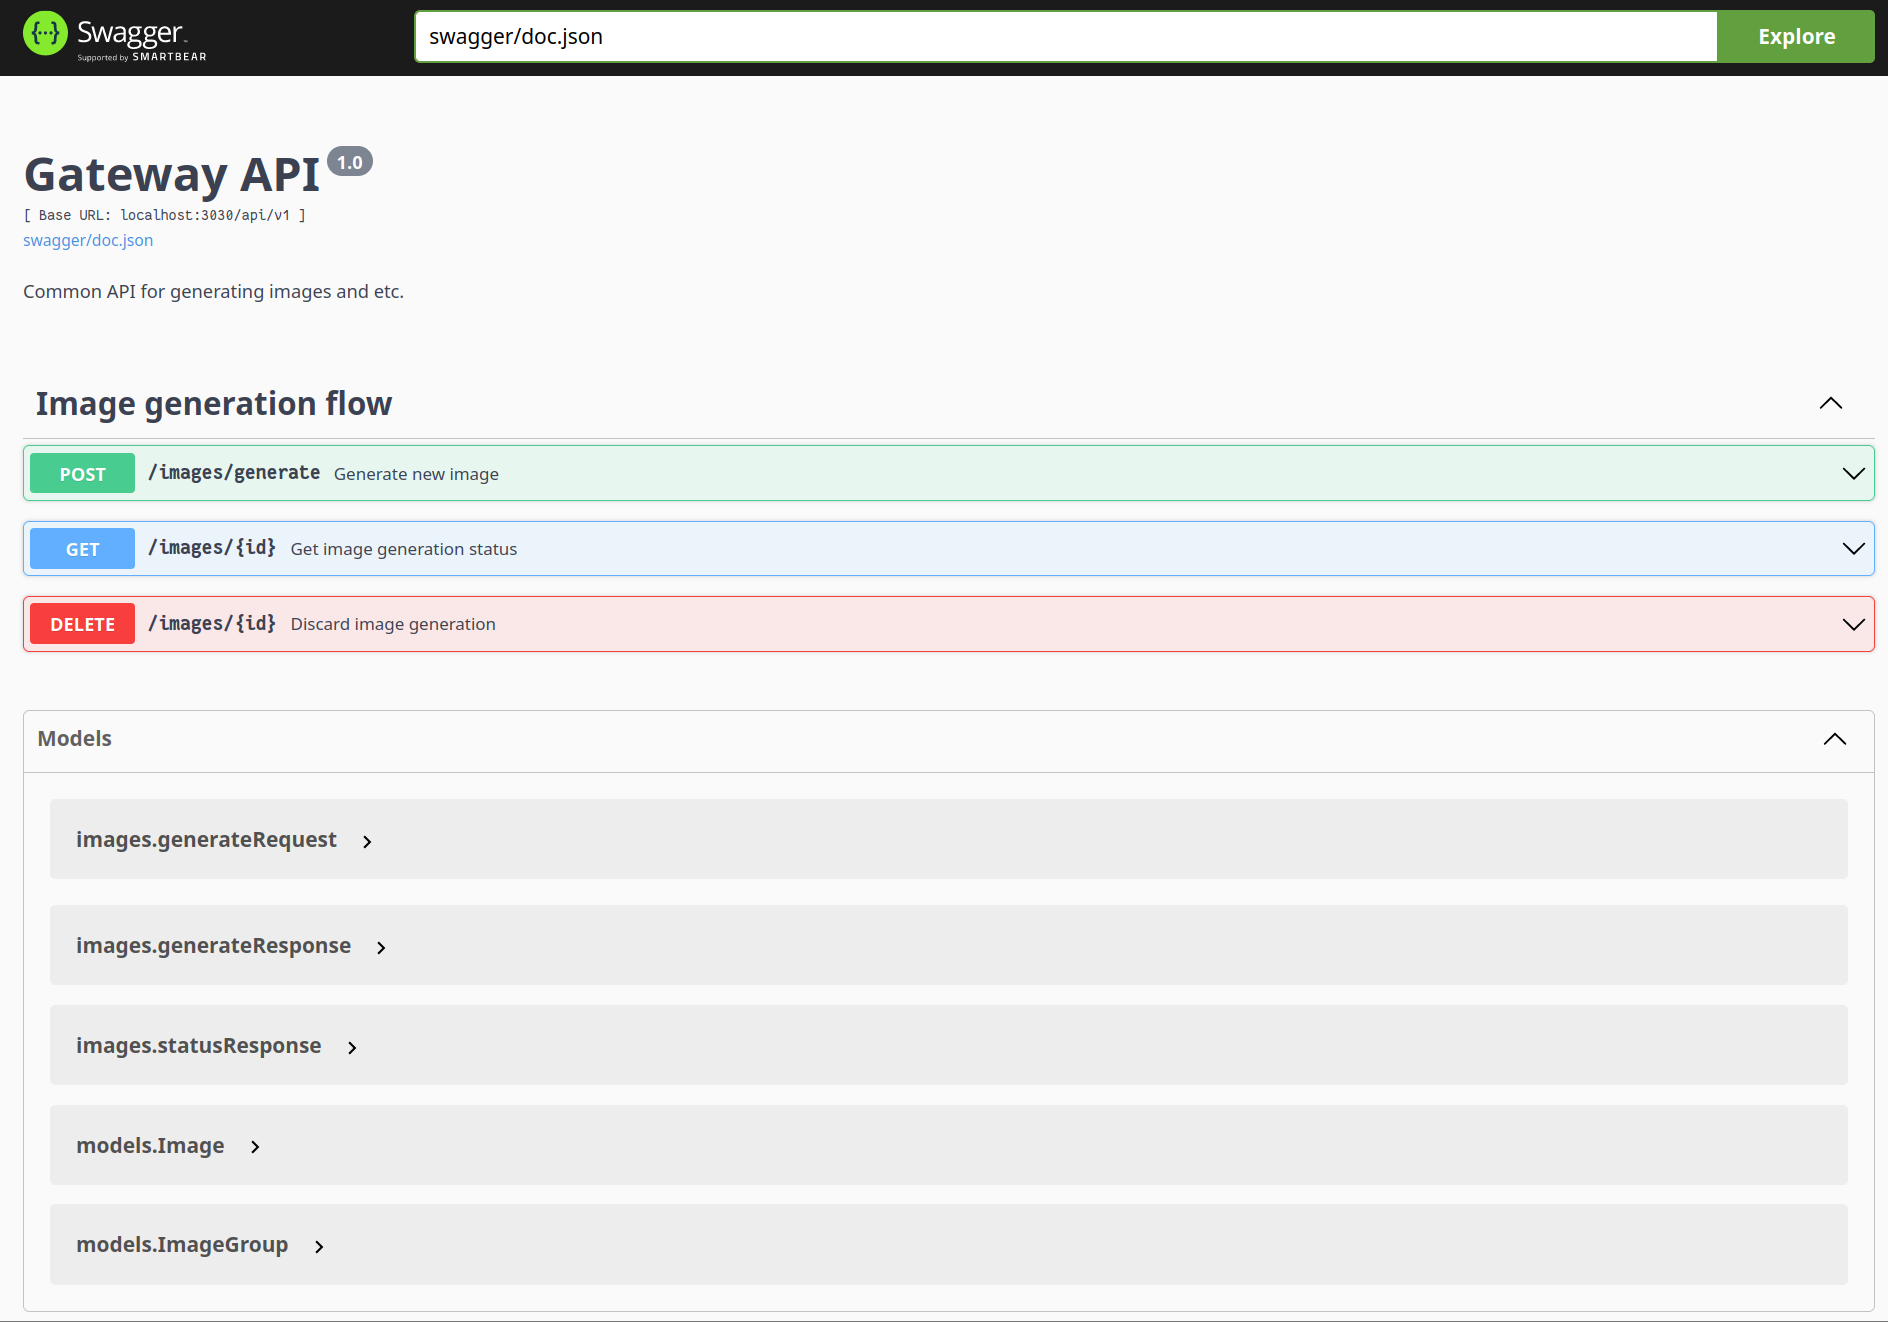
\includegraphics[width=0.95\textwidth]{img/swag.png}
  \caption{Внешняя документация эндпоинтов API}
    \label{fig:swag}
\end{figure}
\end{footnotesize}

Итого, HTTP Gateway собирает необходимую информацию из пользовательского запроса и осуществляет сетевой
поход по GRPC в основной backend с нужными параметрами.

Основной backend принимает запросы от HTTP-прокси и осуществляет все сетевые походы во внешние сервисы для
их обслуживания. Для хранения информации об активных запросах, которые обрабатываются асинхронно, необходимо персистентное 
хранилище в виде, например, реляционной базы данных. В данном примере используется YDB, которая является реляционной базой данных.
Также при локальных запусках используется SQlite, поскольку она не требует запуска отдельного контейнера
с исполняемым файлом

Помимо текстовых данных в этом узле системы необходимо работать с бинарными данными, например, изображениями, которые
не рекомендуется хранить в реляционных базах данных. Одним из самых популярных вариантов хранения подобных данных
является AWS S3 (Simple Storage Service). Делегирование хранения бинарных статичных данных в подобный сервис позволяет
использовать CDN для кэширования наиболее востребованных файлов, что предоставляет оптимальное время загрузки данных на клиенте.

Внутренний backend приводит пользовательские HTTP запросы в версионируемые сообщения в Protobuf формате и
записывает в SQS очередь, которую читает сайдкар генерации. Сайдкар генерации занимается непосредственным общением
с моделью нейронной сети, которые зачастую требуют GPU ресурсы, которые менее доступны, чем CPU и RAM, поэтому
количество сайдкаров можно масштабировать назависимо от основного backend-а по количеству доступных GPU.

При реализации взаимодействия между потребителем очереди, который может быть написан на платформе, отличной
от рантайма инференса, возникают различные варианты реализации.

В случае наличия биндингов к рантайму инференса сайдкар может не производить межпроцессного взаимодействия
и коммуницировать с моделью прямо в памяти (рис \ref{fig:side1}). Подобные варианты возможны при использовании 
общеизвестных рантаймов, типа TRT, Onnx и так далее, поскольку биндинги доступны для большого числа платформ.
Однако это требует сохранения модели в установленном формате, что не всегда подходит для произвольной модели.


\begin{footnotesize}
\begin{figure}[H]
  \centering
  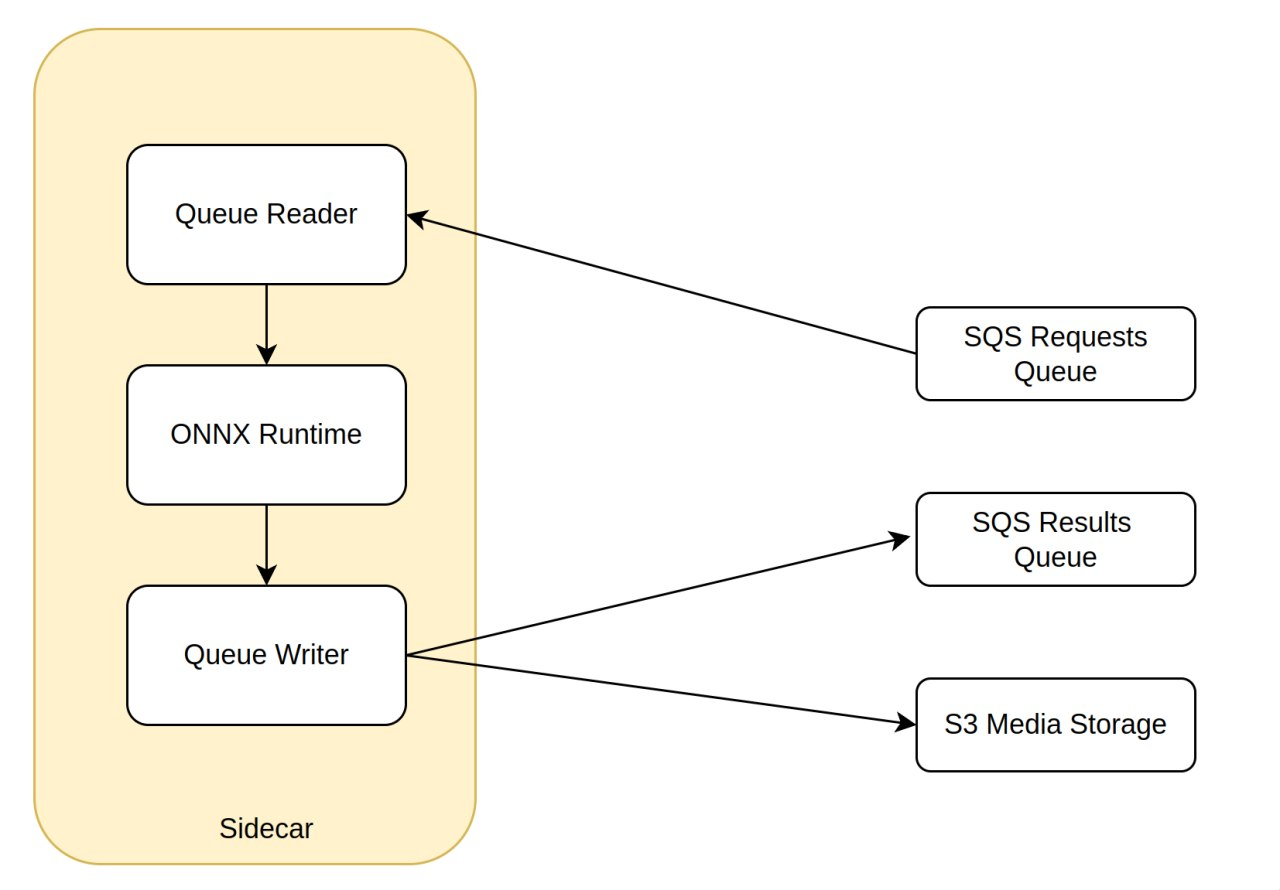
\includegraphics[width=0.95\textwidth]{img/side1.jpg}
  \caption{Нативный способ общения с моделью}
    \label{fig:side1}
\end{figure}
\end{footnotesize}

В случаях, когда отсутствует реализация биндигов рантайма модели к основному языку бэкенда,
можно прибегнуть к сетевой передаче данных по HTTP (рис. \ref{fig:side2}). Достоинство данного метода
заключается в простоте использования и внедрения. Данный подход не требует особого формата модели и может
быть использован с верхнеуровневым кодом инференса. В то же время данный подход может не подойти
в ситуациях, где предъявляются строгие требования к latency запросов, потому что передача крупных
бинарных файлов медленнее передачи их по памяти процесса.

\begin{footnotesize}
\begin{figure}[H]
  \centering
  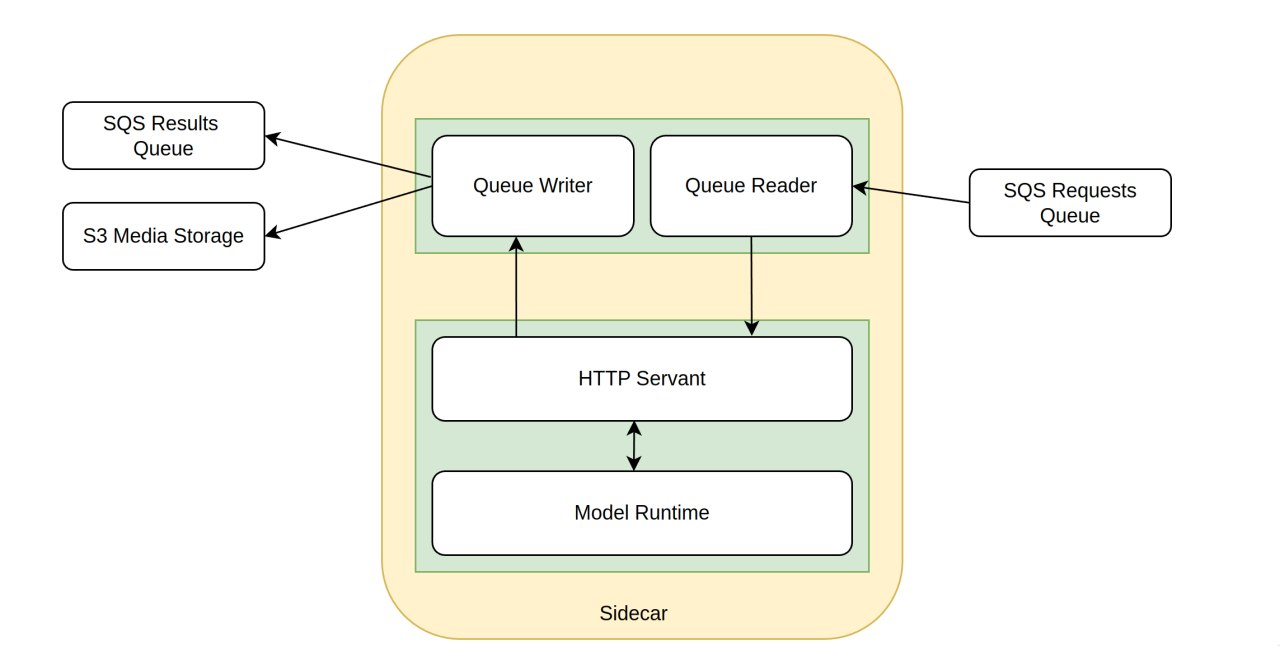
\includegraphics[width=0.95\textwidth]{img/side2.jpg}
  \caption{Общение по HTTP с моделью}
    \label{fig:side2}
\end{figure}
\end{footnotesize}

Еще одним способом передачи данных по сети является общение по UDS (рис. \ref{fig:side3}), которое семантически похоже
на общение по TCP c точностью до того, что транспорт данных осуществляется непосредственно через 
память ядра операционной системы. Данный способ показывает многократное улучшение в таймингах ответов
по сравнению с передачей данных по HTTP, однако требует реализации сообственного бинарного протокола, что 
затрудняет разработку.

\begin{footnotesize}
\begin{figure}[H]
  \centering
  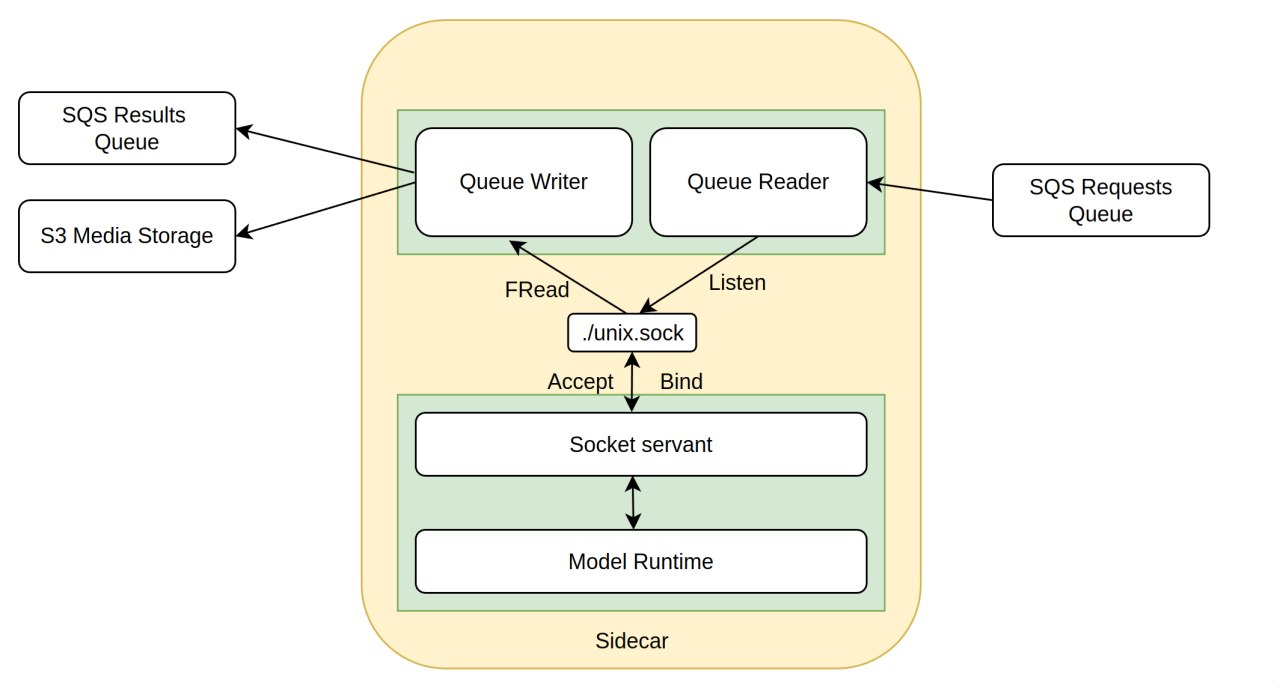
\includegraphics[width=0.95\textwidth]{img/side3.jpg}
  \caption{UDS общение с моделью}
    \label{fig:side3}
\end{figure}
\end{footnotesize}

В данном приложении используется взаимодействие через оперативную память, так как
доступен вариант с нативными привязками для Stable Diffusion, которая представляет собой
латентную диффузионную модель.
Инференс Stable Diffusion реализован через C++ библиотеку на основе ggml, что позволяет производить
оптимизированные вычисления на центральном процессоре без видеокарты.
Привязка к собранной библиотеке под C++ для языка Golang осуществляется через поставляемые 
объектные файлы. Данный подход обеспечивает максимальную производительность, но требует 
обработки соглашений вызовов и бинарных API каждой операционной системы. 

В качестве альтернативы применяется также инструмент CGO для языка Golang, который позволяет описывать
символы кода под язык C прямо в коде программ на Golang, что упрощает сборку и разработку, но налагает
значительные ограничения и требует дополнительных ресурсов при переключении контекста между
вызовами процедур на разных языках.

Локальная разработка без выделенных GPU ресурсов обеспечивается за счет уменьшения шагов семплирования
и понижения разрешения изображения, которое необходимо сгенерировать. В случаях, когда не требовалось
использование реальной модели для исследования ее влияния на всю остальную систему, использовался
отдельный интерфейс, который отдавал заготовленные изображения.

\section{Сценарии использования системы генерации изображений}
По умолчанию запрос на генерацию состоит из следующих шагов:
\begin{enumerate}
  \item Клиент отправляет POST запрос с промптом и параметрами изображения.
  \item HTTP Gateway собирает GRPC запрос и вызывает удаленную процедуру внутреннего backend-а.
  \item Внутренний backend создает запись в реляционной базе данных и кладет запрос на генерацию в очередь сайдкара.
  \item Сайдкар достает запрос из очереди и осуществляет инференс модели.
  \item Полученное изображение перекладывается в S3, а ссылка вместе с индентификаторами генерации отправляется в ответную очередь.
  \item При поступлении ответного сообщения изображение перекладывается из временного бакета S3 в публичный, а у генерации в базе данных обновляется статус.
  \item Клиент, получив идентификатор генерации, осуществляет поллинг хендлера статуса до подтверждения завершения, и в конце получает ссылку на полученнное изображение.
\end{enumerate}

Гарантии на обработку сообщения осуществляются за счет Aknowledge семантики чтения сообщений из очереди. 
В SQS это реализовано через выставление visibility timeout, в течение которого сообщение не может быть заново прочитано другим
потребителем. При успешной обработке сообщение удаляется из очереди. При неуспешной обработке сообщение снова становится 
видим для других потребителей и повторно обрабатывается до удаления из очереди.

При возникновении неопределенного поведения или возникновения неконсистентности данных статус может не обновиться.
Для этого предлагается установить TTL на таблицы, связанные с хранением данных о генерации, для 
возможности проставления соответствующего HTTP статуса в API.

В случае, когда время обработки сообщений превышает интервал, с которым в систему
поступают новые запросы, сообщения становятся в очередь, и время обработки сообщения будет 
включать не только время непосредственной обработки, но и время пребывания в очереди.

Для масштабирования поступающей нагрузки необходимо увеличивать количество сайдкаров, которые могут 
обрабатывать очередь независимо друг от друга. Так же уменьшение времени обработки сообщения можно 
достичь за счет батчевания поступающих сообщений: подобная обработка увеличивает время обработки 
каждого отдельного сообщения, но дает выигрыш для группы сообщений, что увеличивает общую
пропускную способность системы.

Как было описано выше, при использовании батчинга можно обрабатывать несколько сообщений одновременно (рис. \ref{fig:flame1})
Однако в этой схеме остаются блокирующие io операции, которые удерживают ресурс GPU во время сборки сообщения и отправки изображений
в S3. 

\begin{footnotesize}

\begin{figure}[H]
  \centering
  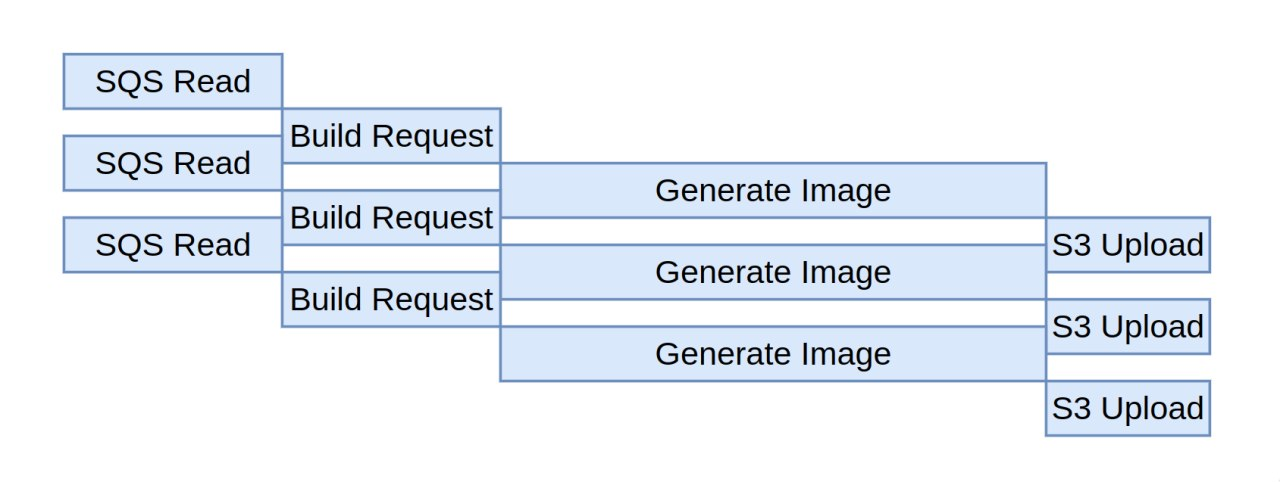
\includegraphics[width=0.95\textwidth]{img/flame1.jpg}
  \caption{Батчевая обработка сообщений}
    \label{fig:flame1}
\end{figure}
\end{footnotesize}

Во избежание простоя GPU между отправкой сообщений можно захватывать сообщения наперед
и отправлять их на генерацию во время отправки в S3 (рис. \ref{fig:flame2}).
Данная оптимизация может сэкономить до 200 мс при ожидании в очереди, что составляет
около 5\% от времени генерации изображения в разрешении 256х256 на видеокарте Nvidia Tesla V100.

\begin{footnotesize}
\begin{figure}[H]
  \centering
  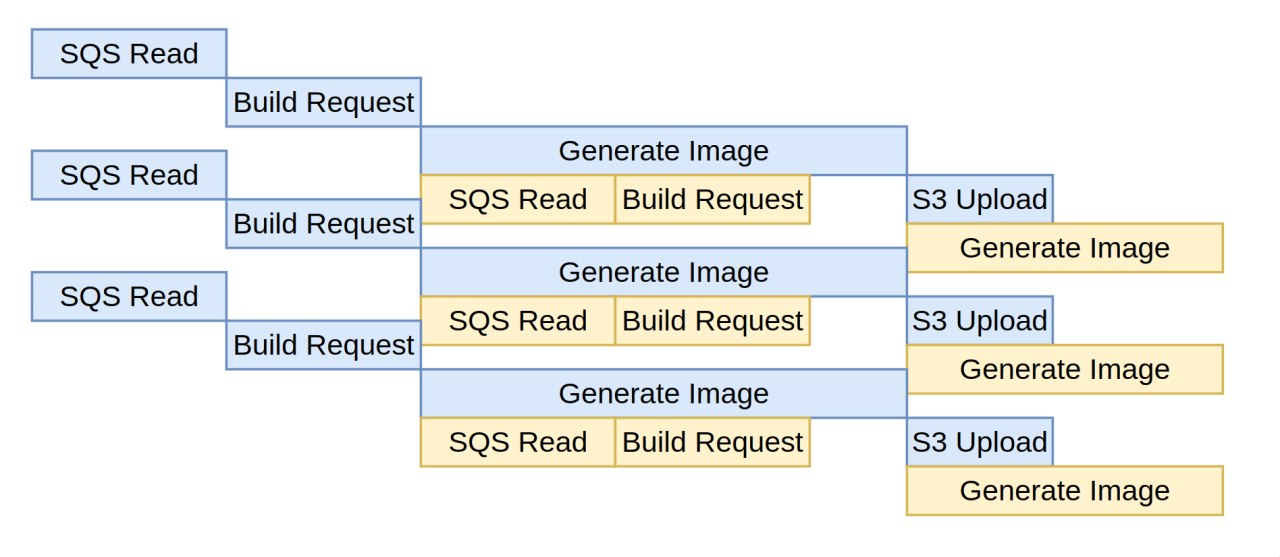
\includegraphics[width=0.95\textwidth]{img/flame2.jpg}
  \caption{Батчевая обработка сообщений с захватом очереди}
    \label{fig:flame2}
\end{figure}
\end{footnotesize}